\section*{Introduktion}
\label{Introduktion}
%
Formålet med dette miniprojekt er, at anvende metoden \textit{Multidimensional Scaling}, (MDS), til at analysere data indsamlet i et eksperiment, hvor 13 forskellige ansigtsudtryk blev præsenteret for testpersonerne. Metoden MDS anvendes, da det giver indblik i hvilke faktorer, der kan have haft betydning for testpersonernes vurderingen af ansigtsudtrykkene, \parencite[p.2]{Wickelmaier2003}. De 13 ansigtsudtryk fremgår af  \autoref{fig:ansigtsudtryk}. 
%
\begin{figure}[H]
\centering
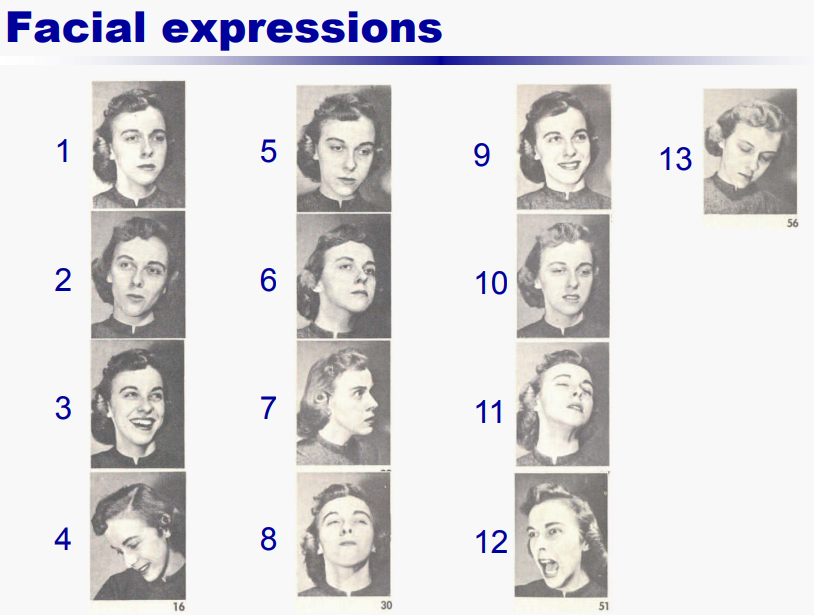
\includegraphics[width = 0.9\textwidth]{Figure/FacialExpressions.PNG} 
\caption{De 13 ansigtsudtryk, der præsenteres for testpersonerne.}
\label{fig:ansigtsudtryk}
\end{figure}
%